\section{Лекция 2}
Напомним формулировки.
Основная задача (будет решена в следующем семестре):
\begin{equation}
    \begin{cases}
        \dot{x} = f(x, u), \quad x \in E^n, \; u \in E^m  \\
        x(t_0) \in M_0 \subset E^n \\
        x(t_1) \in M_1 \subset E^n \\
        \displaystyle J[u] = \int\limits_{t_0}^{t_1} f^0(x, u) \, dt \rightarrow \min\limits_{u \in D_U}, \quad U \subset E^m
    \end{cases}
\end{equation}

Упрощённая задача~--- задача линейного быстродействия:
\begin{equation}
    \begin{cases}
        \dot{x} = Ax + u \\
        x(t_0) \in M_0 \subset E^n \\
        x(t_1) \in M_1 \subset E^n \\
        J = t_1 - t_0 \rightarrow \min\limits_{u \in D_U}, \quad U \subset E^n
    \end{cases}
\end{equation}

Приведём ещё один пример задачи, описываемой линейной системой.

\subsection{Модель пружинного маятника}
\begin{center}
    \begin{tikzpicture}
        % Axe and walls
        \draw [->] (-8,0) -- (8, 0) node [right] {$x$};
        \draw [fill = black] (0,0) circle[radius = 1pt] node [below] {$0$};
        \draw (-7, 0) -- (-7, 3);
        \draw (7, 0) -- (7, 3);

        % Ball
        \draw (-3, 1) circle [radius = 10mm];
        \node [above] at (-3, 2) {$m$};
        \fill [black] (-3, 0) circle[radius = 1pt] node [below] {$x_0$};

        % Spring
        \draw [
        line join = round, 
        decorate, 
        decoration = {
            zigzag, 
            segment length = 10, 
            amplitude = 5,
            post length = 5mm
        }] (-7, 1) -- (-4, 1);

        % Forces
        \draw [green] (-4, 1) circle[radius = 1pt];
        \draw [-latex, thin, green!70!black] (-4, 1) -- (-1.5, 1) node [right] {$F_{\text{упр}}$}; 
        \fill [blue] (-3, 1) circle [radius = 1pt];
        \draw [-latex, thin, blue] (-3, 1) -- (-2.25, 1) node [anchor = south east] {$F$};
        
    \end{tikzpicture}
\end{center}

Запишем второй закон Ньютона для пружинного маятника, на который действует сила упругости $F_{\text{упр}} = -kx$ и внешняя сила $F$.
\begin{equation}
    m\ddot{x} = -kx + F
\end{equation}

Опять же, хотим доставить маятник в точку $x = 0$ и остановить его там.
\begin{equation}
    \begin{array}{cc}
        x(t_0) = x_0, & \dot{x}(t_0) = x_{01} \\
        x(t_1) = 0, & \dot{x}(t_1) = 0
    \end{array}
\end{equation}

Преобразуем уравнение:
\begin{equation}
    \ddot{x} = -\frac{k}{m}x + \frac{F}{m}
\end{equation}

Сделаем замены $\cfrac{k}{m} = \omega^2, \; \cfrac{F}{m} = v$.
Для простоты считаем, что $\omega = 1, |v| \leqslant 1$.

Тогда $\ddot{x} = -x + v$.
Как и в прошлой задаче, введём переменные ${x_1 = x}, \; {x_2 = \dot{x}}$.
Тогда 
\begin{align}
    \label{lection2:pendulum}
    \dot{x_1} = x_2, \\
    \dot{x_2} = -x + v
\end{align}

Обозначим ${\vec{u} = \left( \begin{matrix} u_1 \\ u_2 \end{matrix} \right)} = \left( \begin{matrix} 0 \\ v \end{matrix} \right) $,
а также $A = \left(
    \begin{matrix}
        0 & 1 \\
        -1 & 0
    \end{matrix}
\right)$.
Тогда можно записать уравнение \ref{lection2:pendulum} в виде
\begin{equation}
    \begin{cases}
        \dot{\vec{x}} = A\vec{x} + \vec{u} \\
        \vec{x}(t_0) = \left(
            \begin{matrix}
                x_0 \\
                x_{01}
            \end{matrix}
        \right) \\
        \vec{x}(t_1) = \left(
            \begin{matrix}
                0 \\
                0
            \end{matrix}
        \right) \\
        t_1 - t_0 \rightarrow \min\limits_{u \in D_U}
    \end{cases}
\end{equation}

\vspace{1cm}
В этом курсе будут обсуждаться следующие темы:
\begin{enumerate}
    \item Управляемость (т.е. существование хотя бы одного допустимого процесса $\bigl(u(t), x(t)\bigr)$ (т.е. эта штука вообще управляется?))
    \item Теоремы существования.
    \item Необходимые условия оптимальности.
    \item Достаточные условия оптимальности.
    \item Теоремы единственности.
\end{enumerate}

\subsection{Элементы выпуклого анализа}

В евклидовом пространстве $E^n$ есть скалярное произведение $(x, y) = \sum\limits_{i = 1}^{n} x_i y_i$.
Это позволяет нам ввести метрику и расстояние:
\begin{align}
    \Norm{x} = \sqrt{(x,x)} \\
    \rho(x, y) = \Norm{x-y}
\end{align}

\begin{defn}
    \label{lection2:ball}
    Замкнутым шаром в $E^n$ называется множество
    \begin{equation}
        S_r(a) = \bigl\{ x \in E^n \colon \Norm{x - a} \leqslant r \bigr\}.
    \end{equation}
\end{defn}

А кроме того, ещё целый блок определений, касающийся свойств множеств в $E^n$.
\begin{enumerate}
    \item $f$~--- \textit{внутренняя} точка множества $F \in E^n$, если $\exists \, \varepsilon > 0\colon S_\varepsilon(f) \subset F$.
    \item $\operatorname{int} F$~--- множество всех внутренних точек множества $F$ (или \textit{внутренность} множества $F$).
    \item $f$~--- \textit{предельная} точка множества $F \in E^n$, если $\forall \, \varepsilon > 0 \; S_\varepsilon(f) \cap F \neq \varnothing$.
    \item $F$~--- \textit{замкнутое} множество, если оно содержит все свои предельные точки.
    \item $\overline{F}$~--- минимальное замкнутое множество, содержащее $F$ (или \textit{замыкание} множества $F$).
    \item $\partial F = F \setminus \operatorname{int} F$~--- \textit{граница} множества $F$.
    \item $F$ ограничено, если $\exists \, R > 0\colon F \subset S_R(0)$.
    \item Ограниченное и замкнутое множество в $E^n$~--- компакт.
    \item $\Omega(E^n)$~--- множество непустых компактов в $E^n$.
    \item Пусть $a, b \in E^n$. Тогда $[a, b] = \bigl\{ x \in E^n \SuchThat x = \lambda a + (1 - \lambda)b, \; \lambda \in [0,1] \bigr\}$.
    \item Множество $F$ называется выпуклым, если $\forall \, a, b \in F \implies [a, b] \subset F$.
    \item Пусть $F \in E^n$. Тогда $\operatorname{conv} F$~--- минимальное выпуклое множество, содержащее $F$ (\textit{минимальная выпуклая оболочка}).
    \item $\operatorname{conv} \Omega(E^n)$~--- множество непустых выпуклых компактов в $E^n$.
    \item \textit{Модуль} множества $F \in \Omega(E^n)\colon |F| = \max\limits_{x \in F} |x|$.
    Для ограниченного $F$~--- $|F| = \sup\limits_{x \in F} |x|$.
\end{enumerate}

\begin{defn}
    Пусть $F_1, F_2 \in \Omega(E^n)$.
    Введём операцию сложения множеств:
    \begin{equation*}
        F_1 + F_2 = \bigl\{f = f_1 + f_2 \SuchThat f_1 \in F, \; f_2 \in F\bigr\}.
    \end{equation*}
\end{defn}

\begin{exmp}
    Пусть $F_1 = \{f_1\} \subset E^n$, $F_2 \in \Omega(E^n)$.
    Тогда $F_1 + F_2 = f_1 + F_2$~--- параллельный перенос на вектор $f_1 \in E^n$.
\end{exmp}

\begin{exmp}
    Пусть $F_1 = \bigl\{f \in E^2 \colon f_1 = 0, |f_2| \leqslant 1 \bigr\}$, \\
    $F_2 = \bigl\{f \in E^2 \colon |f_1| \leqslant 1, f_2 = 0 \bigr\}$~--- отрезки. \\
    Тогда $F_1 + F_2 = \bigl\{f \in E^2 \colon |f_1| \leqslant 1, |f_2| \leqslant 1 \bigr\}$~--- квадрат. 
    \begin{center}
        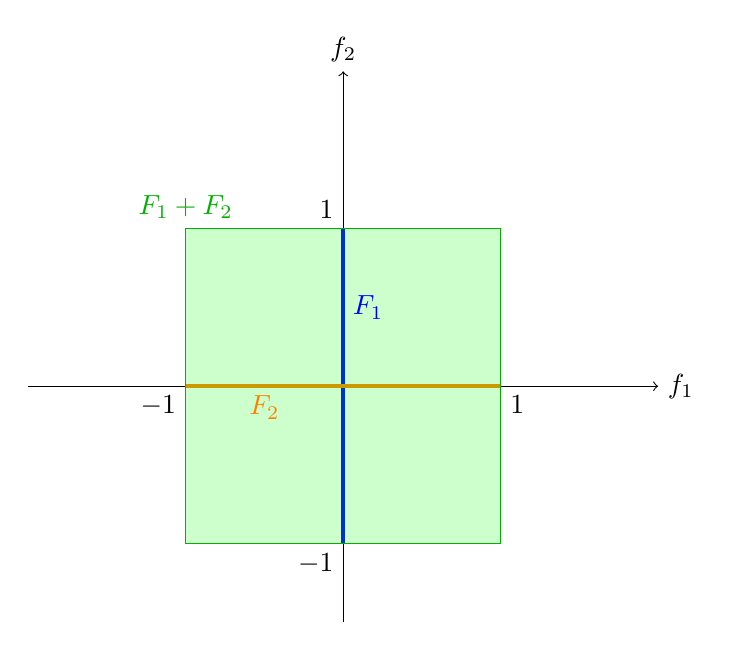
\begin{tikzpicture}
            % Axes
            \draw [->] (0,-3) -- (0, 4) node [above] {$f_2$};
            \draw [->] (-4,0) -- (4, 0) node [right] {$f_1$};
    
            % Draw sets: F_1, F_2 and F_1 + F_2 respectively
            \draw [ultra thick, blue] (0, -2) -- (0, 2);
            \draw [ultra thick, orange] (-2, 0) -- (2, 0);
            \draw [draw = green!70!black, fill = green, fill opacity = 0.2] (-2, -2) rectangle (2, 2);
    
            % Some coordinates
            \node[anchor = north east] at (-2, 0) {$-1$};
            \node[anchor = north west] at ( 2, 0) {$ 1$};
            \node[anchor = north east] at (0, -2) {$-1$};
            \node[anchor = south east] at (0,  2) {$1$};
    
            % Subsript set names
            \node[blue, anchor = west] at (0, 1) {$F_1$};
            \node[orange, anchor = north] at (-1, 0) {$F_2$};
            \node[green!70!black, anchor = south] at (-2, 2) {$F_1 + F_2$};
        \end{tikzpicture}
    \end{center}
    \begin{rmrk}
        \textit{Здесь $f_1$ и $f_2$~--- первая и вторая координаты двумерного вектора, а не элементы множеств $F_1$ и $F_2$, как было в определении суммы множеств.}
    \end{rmrk}
\end{exmp}

\begin{exmp}
    Пусть $F_1 = S_{r_1}(a_1), \; F_2 = S_{r_2}(a_2)$.
    Тогда $F_1 + F_2 = S_{r_1 + r_2}(a_1 + a_2)$.
    \begin{center}
        \begin{tikzpicture}
            % Axes
            \draw [->] (0,-4) -- (0, 5) node [above] {$f_2$};
            \draw [->] (-2,0) -- (8, 0) node [right] {$f_1$};
    
            % Create centers of balls and the (0, 0) point
            \coordinate (Origin) at (0, 0);
            \coordinate (CenterFirst) at (2, 4);
            \coordinate (CenterSecond) at (4, -2);
            \coordinate (CenterThird) at ($(CenterFirst) + (CenterSecond)$);

            % Draw balls with given color and radius
            \draw [fill = blue] (CenterFirst) circle[radius = 6mm];
            \draw [fill = orange] (CenterSecond) circle[radius = 9mm];
            \draw [fill = green] (CenterThird) circle[radius = 15mm];
            % \draw [draw = orange] (CenterThird) circle[radius = 9mm]; --- maybe should have drawn a circle inside big one but idk

            % Draw radius-vectors
            \draw [-latex] (0,0) -- (CenterFirst);  
            \draw [-latex] (0,0) -- (CenterSecond); 
            \draw [-latex] (0,0) -- (CenterThird);
            % And two more vectors to form a parallelogram
            \draw [-latex, dashed] (CenterFirst) -- (CenterThird);
            \draw [-latex, dashed] (CenterSecond) -- (CenterThird);

            % Write subscripts for radius-vectors halfway to the ball center
            \node [anchor = south east] at ($(Origin)!.50!(CenterFirst)$) {$\vec{a_1}$};
            \node [anchor = south west] at ($(Origin)!.50!(CenterSecond)$) {$\vec{a_2}$};
            \node [anchor = south east] at ($(Origin)!.50!(CenterThird)$) {$\vec{a_1} + \vec{a_2}$};

            % Draw ball's radii and their subscripts
            \draw [-latex] (CenterFirst) -- ($ (CenterFirst) + (120 : 0.6)$) node [anchor = south] {$r_1$};
            \draw [-latex] (CenterSecond) -- ($ (CenterSecond) + (300 : 0.9)$) node [anchor = north] {$r_2$};
            \draw [-latex] (CenterThird) -- ($ (CenterThird) + (90 : 1.5)$) node [anchor = south] {$r_1 + r_2$};

            % Subscript set names
            \node [blue, anchor = west] at ($ (CenterFirst) + (30 : 0.6)$) {$F_1$};
            \node [orange!70!black, anchor = west] at ($ (CenterSecond) + (30 : 0.9)$) {$F_2$};
            \node [green!70!black, anchor = west] at ($ (CenterThird) + (30 : 1.5)$) {$F_1 + F_2$};

        \end{tikzpicture}
    \end{center}

    Докажем это.
    Для того, чтобы показать равенство произвольных множеств $A$ и $B$, достаточно доказать двустроннее вложение: 
    $A \subset B$ и $B \subset A$.
    \begin{itemize}
        \item 
            $S_{r_1}(a_1) + S_{r_2}(a_2) \subset S_{r_1 + r_2}(a_1 + a_2)$. 

            Возьмём произвольный $f \in S_{r_1}(a_1) + S_{r_2}(a_2)$.
            По определению суммы множеств это значит, что существуют такие $g \in S_{r_1}(a_1), h \in S_{r_2}(a_2)$, что $g + h = f$.
            Тогда 
            \begin{equation*}
                \Norm{f - a_1 - a_2} = \Norm{g + h - a_1 - a_2} \leqslant \Norm{g - a_1} + \Norm{h - a_2} \leqslant r_1 + r_2.
            \end{equation*}
            Таким образом, $f \in S_{r_1 + r_1}(a_1 + a_2) = \bigl\{f \in E^n \colon \Norm{f - a_1 - a_2} \leqslant r_1 + r_2 \bigr\}$.
            В силу произвольности выбора $f$ получаем, что $S_{r_1}(a_1) + S_{r_2}(a_2) \subset S_{r_1 + r_2}(a_1 + a_2)$.
        \item 
            $S_{r_1 + r_2}(a_1 + a_2) \subset S_{r_1}(a_1) + S_{r_2}(a_2)$.

            Возьмём произвольный $f \in S_{r_1 + r_2}(a_1 + a_2)$.
            Легко видеть, что ${\tilde{f} = f - a_1 - a_2 \in S_{r_1 + r_2}(0)}$:
            \begin{equation*}
                \Norm{\tilde{f}} = \Norm{f - a_1 - a_2} \leqslant r_1 + r_2.
            \end{equation*}
            Положим теперь 
            \begin{equation*}
                \tilde{g} = \frac{r_1}{r_1 + r_2} \tilde{f}, \;\; \tilde{h} = \frac{r_2}{r_1 + r_2} \tilde{f}.
            \end{equation*}
            Очевидно, что $\tilde{g} + \tilde{h} = \tilde{f}$.
            При этом $\tilde{g} \in S_{r_1}(0)$, ведь $\Norm{\tilde{g}} = \cfrac{r_1}{r_1 + r_2}\Norm{\tilde{f}} \leqslant \cfrac{r_1}{r_1 + r_2} (r_1 + r_2) = r_1$.
            Аналогично $\tilde{h} \in S_{r_2}(0)$.

            Если мы введём $g$ и $h$ как 
            \begin{equation*}
                g = \tilde{g} + a_1, \; h = \tilde{h} + a_2
            \end{equation*}
            то $g \in S_{r_1}(a_1), \; h \in S_{r_2}(a_2)$ и 
            \begin{equation*}
                g + h = \tilde{g} + \tilde{h} + a_1 + a_2 = \tilde{f} + a_1 + a_2 = f - a_1 - a_2 + a_1 + a_2 = f
            \end{equation*}
            Но это значит, что $f \in S_{r_1}(a_1) + S_{r_2}(a_2)$.
            В силу произвольности $f$ заключаем, что $S_{r_1 + r_2}(a_1 + a_2) \subset S_{r_1}(a_1) + S_{r_2}(a_2)$.
    \end{itemize}
\end{exmp}